\subsection{Asymptotic approximation}
Eq\ref{eq:explicitL} can be annoying to work with, especially for large $h$, so an approximation for the case $h \gg m$ is needed. Intuitively the length of a fight should have linear dependency on hitpoints as $h \rightarrow \infty$. This is because on average one can expect each hit to do $am/2$ damage and therefore it should take approximately $2h/am$ hits to kill an enemy with $h$ hitpoints. Due to overkill however, the last hit will do slightly less than $am/2$ damage on average introducing a constant correction term to this linear approximation.
%Since eq\ref{eq:explicitL} is tricky to approximate we take a completely different approach and try to look at the damage per hit directly instead of trying to approximate $\L_h$. Recall the definition of a fight as a sequence of damage rolls $\{X_i\}$. The total damage dealt by these hits is $\sum X_i = h$, but because of overkill the last hit contributes less to this sum than the others. To find the magnitude of this discrepancy, let us ignore all the hits that deal no damage to obtain a sequence of non-zero hits, $\{Z_i\}$. This is a subsequence of $\{X_i\}$ and its elements have the following probabilities, where $H_i$ is the remaining hitpoints after $i$ \textit{non-zero} hits.
%\begin{align}
%    \Pr{Z_i = k \mid H_{i-1} = l} = \begin{cases}
%        \frac{1}{m}, &\quad\mbox{if } k < l\\
%        \frac{m-k+1}{m}, &\quad\mbox{if } k = l\\
%        0, &\quad\mbox{if } k > l \quad \mbox{or } k \notin [1,m]
%    \end{cases}
%\end{align}
%The probability distribution of $H_i$ is given recursively for $i \geq 1$ and $k > 0$.
%\begin{align}
%    \Pr{H_i = k} &= \sum_{j\geq 1} \Pr{Z_i = j \mid H_{i-1} = k+j}\Pr{H_{i-1} = k+j} = \frac{1}{m}\sum_{j=1}^m \Pr{H_{i-1} = k+j}
%\end{align}
%The case $k=0$ is interesting since $\Pr{H_i = 0} = \Pr{L_h = i}$. This is given by
%\begin{align}
%    \Pr{H_i = 0} &= \sum_{j\geq 1} \Pr{Z_i = j \mid H_{i-1} = j}\Pr{H_{i-1} = j} = \sum_{j=1}^m \frac{m-j+1}{m}\Pr{H_{i-1} = k+j}
%\end{align}
%Since every fight starts at $h$ hitpoints the inital condition is $\Pr{H_0=k} = \delta_{k,h}$, where $\delta_{k,h}$ is the Kronecker delta.
%
%We say that the state $k$ is visited if there exists $i \in \mathbb{N}_0$ such that $H_i = k$. This is the same as saying that at some point during the fight the enemy had $k$ hitpoints remaining. Let $\Pr{V_k}$ be the probability of visiting state $k$. For the initial and final states we have $\Pr{V_h} = \Pr{V_0} = 1$ and between them the visiting probability can be specified recursively.
%\begin{align}
%    \Pr{V_k} &= \sum_{i \geq 0} \Pr{H_i = k} = \frac{1}{m}\sum_{j=1}^m \sum_{i \geq 0} \Pr{H_{i-1} = k+j}\nonumber\\
%            &= \frac{1}{m}\sum_{j=1}^m \left(\Pr{H_0 = k+j} + \sum_{i \geq 1} \Pr{H_{i-1} = k+j}\right)\nonumber\\
%            &= \frac{1}{m}\sum_{j=1}^m \left(\delta_{k+j,h} + \sum_{i \geq 0} \Pr{H_{i} = k+j}\right)
%            = \frac{1}{m}\sum_{j=1}^m \left(\delta_{k+j,h} + \Pr{V_{k+j}}\right)\label{eq:vkgen}
%\end{align}
%
%The plan is now to show the existence and find the value of the limit of $\Pr{V_k}$ as $h \rightarrow \infty$ for any fixed $k$. First, we claim that $\Pr{V_k}$ increases as $k$ decreases. Clearly this is not true for the initial state $k=h$ because it is always visited, but for all the lower states we should have
%\begin{claim}\label{claim:vkhinc}
%    $\Pr{V_{k-1}} > \Pr{V_k}$ \quad for $0 < k < h$.
%\end{claim}
%\begin{proof}
%Eq\ref{eq:vkgen} gives
%\begin{align}
%    \Pr{V_{k-1}} &= \frac{1}{m}\sum_{j=1}^m \left(\delta_{(k-1)+j,h} + \Pr{V_{(k-1}+j})\right)\label{eq:proof321}.
%\end{align}
%Consider the case $h - m < k < h$. If $k-1+j > h$ then $\Pr{V_{k-1+j}} = 0$ since the hitpoints of the enemy can never exceed $h$. Therefore, the terms in eq\ref{eq:proof321} for which $j>h-(k-1)$ can be dropped.
%The sum over the Kronecker deltas can be evaluated by noticing that for any $k$ in the range under consideration there is exactly one $j$ for which $k-1+j = h$. With these remarks eq\ref{eq:proof321} can be written as
%\begin{align}
%    \Pr{V_{k-1}} &= \frac{1}{m}\left(1 + \sum_{j=1}^{h-(k-1)}\Pr{V_{(k-1}+j})\right)
%    = \frac{1}{m}\left(1 + \Pr{V_{k}} + \sum_{j=2}^{h-k+1}\Pr{V_{k-1+j}}\right)\nonumber\\
%              &= \frac{1}{m}\left(1 + \Pr{V_{k}} + \sum_{j=1}^{h-k}\Pr{V_{k+j}}\right)\nonumber
%              = \frac{1}{m}\Pr{V_{k}} + \frac{1}{m}\left(1 + \sum_{j=0}^{h-k}\Pr{V_{k+j}}\right)\\
%              &= \frac{1}{m}\Pr{V_{k}} + \Pr{V_{k}} \quad > \quad \Pr{V_{k}}.\label{eq:proof323}
%\end{align}
%This proves the statement for all $k$ in the range $h-m<k<h$ implying $\Pr{V_{h-m}} > \cdots > \Pr{V_{h-1}}$.
%
%Assume that $\Pr{V_{k}} >\cdots> \Pr{V_{k+m-1}}$ is true for some $k$ in the range $0 < k \leq h-m$. In this range the Kronecker delta terms in eq\ref{eq:proof321} vanish and $\Pr{V_{k}}$ is given as the average of the last $m$ terms.
%\begin{align}
%    \Pr{V_{k-1}} &= \frac{1}{m}\sum_{j=1}^m \Pr{V_{(k-1}+j})
%               = \frac{1}{m}\sum_{j=0}^m \Pr{V_{k+j}}
%               > \frac{1}{m}\sum_{j=0}^{m-1} \Pr{V_{k}} = \Pr{V_{k}}
%\end{align}
%We already proved the assumption $\Pr{V_{k}} >\cdots> \Pr{V_{k+m-1}}$ is true for $k=h-m$. By induction the chain of inequalities can therefore be extended to $\Pr{V_{1}} > \cdots > \Pr{V_{h-1}}$, which proves the claim.
%\end{proof}
%Saying that $k$ is decreasing is equivalent to saying that $h$ is increasing for some fixed $k$. Being a probability $\Pr{V_k}$ is also bounded by 1. Therefore the limit $\Pr{V} = \lim_{h \rightarrow \infty}\Pr{V_{k}}$ exists. To find the value of this limit we look at the event $V'_k$, that state $k$ is never visited (i.e skipped). In practice skipping state $k$ means there must be two successive states $H_i$ and $H_{i-1}$ of the fight such that $H_{i} < k < H_{i-1}$. The probability that state $k$ is skipped by jumping over it from state $k+j$ is
%\begin{align}
%    \Pr{V_{k+j}}\Pr{Z_i > j | H_{i-1} = k+j} = \Pr{V_{k+j}}\sum_{n=j+1}^{m}\frac{1}{m} = \Pr{V_{k+j}}\frac{m-j}{m}.
%\end{align}
%This is true regardless of \textit{when} the hitpoint state was visited (i.e for which $H_i$). Since state $k$ can be skipped by jumping over it from any of the states $\{k+1,\ldots,k+m-1\}$ we can write the probability of never visiting $k$ as
%\begin{align}
%    \Pr{V'_k} = 1-\Pr{V_{k}} = \sum_{j=1}^{m-1}\Pr{V_{k+j}}\frac{m-j}{m}.
%\end{align}
%If $\Pr{V}$ is the limit of $\Pr{V_k}$ as $h \rightarrow \infty$ then
%\begin{align}
%    1-\Pr{V} &= \Pr{V}\sum_{j=1}^{m-1}\frac{m-j}{m}
%           = \Pr{V}\sum_{j=1}^{m-1}\left(1 - \frac{j}{m}\right)
%           = \Pr{V}\left((m-1) - \frac{1}{m}\sum_{j=1}^{m-1}j\right)\nonumber\\
%           &= \Pr{V}\left((m-1) - \frac{1}{m}\frac{m(m-1)}{2}\right)
%           = \Pr{V}\frac{m-1}{2}\nonumber\\
%    \implies 1 &= \Pr{V}\left(\frac{m}{2} - \frac{1}{2} + 1\right) = \Pr{V}\frac{m+1}{2}\nonumber\\
%    \implies \Pr{V} &= \frac{2}{m+1}\label{eq:visitproblimit}
%\end{align}
%
%If the number of non-zero hits is $N$, then $Z_N = X_{L_h}$ because the last hit has to do at least $1$ damage by definition. Its expected value can be calculated from the visiting probabilites.
%\begin{align}
%    \overline{Z}_N &= \sum_{n \geq 1} n \Pr{Z_N = n}
%    = \sum_{n \geq 1} n \Pr{V_n} \Pr{Z_N = n \mid H_{N-1} = n}\nonumber\\
%                    &= \sum_{n=1}^{m} n \Pr{V_n} \frac{m-n+1}{m}
%                    = \frac{1}{m}\sum_{n=1}^{m}\Pr{V_n}\left((m+1)n - n^2\right) \nonumber
%\end{align}
%In the limit that $h \rightarrow \infty$ the visit probabilites will be given by eq\ref{eq:visitproblimit} and the expectation has the following limit.
%\begin{align}
%    \lim_{h \rightarrow \infty}\overline{Z}_N
%              &= \frac{1}{m}\sum_{n=1}^{m}\frac{2}{m+1} \left((m+1)n - n^2\right)
%              = \frac{2}{m(m+1)}\left((m+1)\sum_{n=1}^{m} n - \sum_{n=1}^{m} n^2\right)\nonumber\\
%              &= \frac{2}{m(m+1)}\left(\frac{m{(m+1)}^2}{2} - \frac{m(m+1)(2m+1)}{6}\right)\nonumber\\
%              &= \frac{m+1}{2} - \frac{2m+1}{6}
%              = \frac{3m+3 - 2m-1}{6}
%              = \frac{m+2}{6}\label{eq:lastHitDamage}
%\end{align}
%For all the hits except the last one the expected damage dealt is a constant. Namely
%\begin{align}
%    \overline{X}_i
%        &= \sum_{n \geq 1} n \Pr{X = n}
%        = \sum_{n = 1}^{m} n \frac{a}{m+1}
%        = \frac{a}{m+1}\frac{m(m+1)}{2}
%        = \frac{am}{2}\label{eq:otherHitDamage}
%\end{align}
%Comparing eq\ref{eq:lastHitDamage} and eq\ref{eq:otherHitDamage} tells us how overkill lowers the damage dealt per hit. In particular, notice that the last hit does not depend on accuracy because it has to kill the enemy. If overkill did not happen and the damage rolled by the last hit always exactly brought the enemy hitpoints to $0$ the damage dealt by the last hit would have the expected value $\frac{m}{2}$. Therefore, the extra damage that would have been dealt is $\frac{m}{2}-\frac{m+2}{6}=\frac{m-1}{3}$.
%If the expected damage dealt by all the hits, including the last one, was the one specified by eq\ref{eq:otherHitDamage}, then the hitpoints of the enemy would have to be corrected to $h+\frac{m-1}{3}$. This gives the asymptotic approximation for the average length of a fight.
The average length of a fight with no regeneration has the following asymptotic behaviour (derivation not shown here).
\begin{align}\label{eq:asymptoticAppr}
\L_h \sim \frac{2}{ma}\left(h + \frac{m-1}{3}\right)
\end{align}
The correctness of both the results was validated by comparing them to a computer simulation. The comparison is illustrated in figure~2.
\begin{figure}[t]\label{fig:apprComparison}
    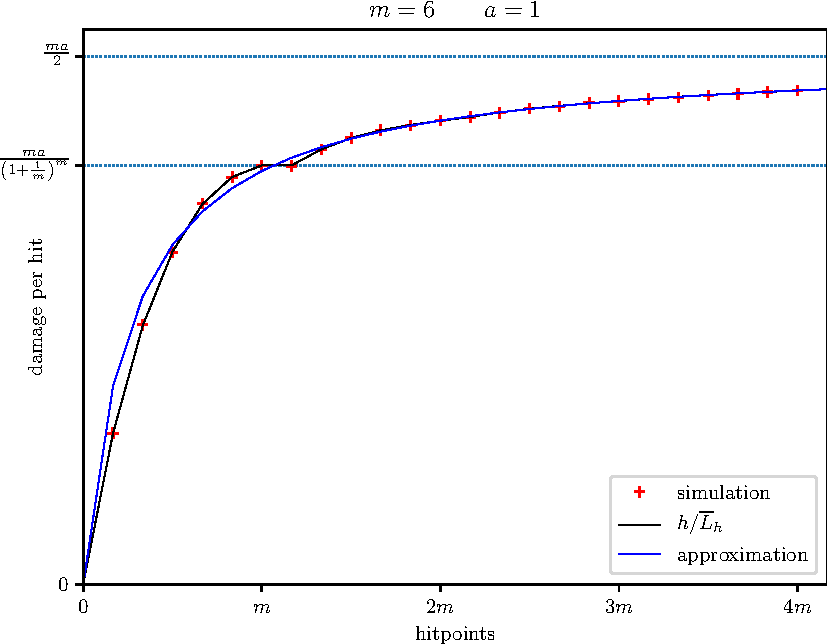
\includegraphics[scale=1.1]{dph-appr-m6.pdf}
    \caption{Comparison of damage per hit (DPH) calculated using the explicit formula (eq\ref{eq:explicitL}), asymptotic approximation (eq\ref{eq:asymptoticAppr}) and a simulation. The simulation was written using the damage calculation mechanics described in Chapter~\ref{chap:fightDef}. For each datapoint $10^{5}$ fights were simulated and their average lengths calculated.}
\end{figure}

%The approximation is clearly correct and converges quite quickly as can be seen from Figure~\ref{fig:apprComparison}. But the lack of rigour in the last few steps of deriving it calls for either a proof of its validity or a different derivation method. If eq\ref{eq:asymptoticAppr} really is an asymptotic approximation of $\L_h$ it should satisfy
%\begin{align}
%    \L_h - \frac{2}{ma}\left(h + \frac{m-1}{3}\right) \xrightarrow[h \rightarrow \infty]{} 0.
%\end{align}
%Unfortunately this could not be proven. One approach to it is using the explicit expression for $\L_h$ given by eq\ref{eq:explicitL}. However, this turns out to be quite tricky due to the binomial coefficients in the sum. It might be necessary to use generating functions or work directly with the defining recurrence relations (eq\ref{eq:complexRecurrence2}). The problem of finding the asymptotic behaviour of the recurrence is a purely mathematical one. Making heavy use of the properties of the underlying problem the recurrence is a solution for should not be necessary.
%\begin{figure}[t]\label{fig:apprComparison}
%    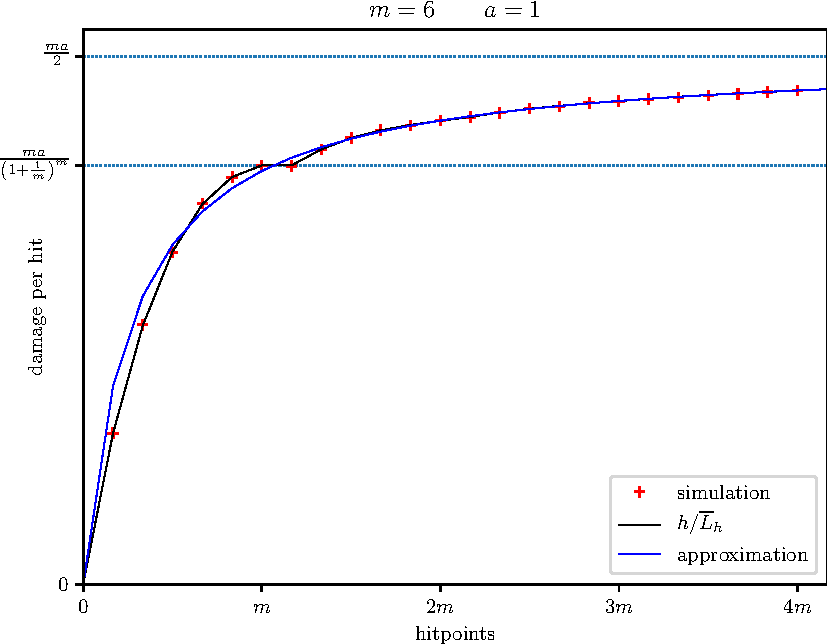
\includegraphics[scale=1.1]{dph-appr-m6.pdf}
%    \caption{Comparison of damage per hit (DPH) calculated using the explicit formula (eq\ref{eq:explicitL}), asymptotic approximation (eq\ref{eq:asymptoticAppr}) and a simulation. The simulation was written using the damage calculation mechanics described in Chapter~\ref{chap:fightDef}. For each datapoint $10^{5}$ fights were simulated and their average lengths calculated.}
%\end{figure}
